% Options for packages loaded elsewhere
\PassOptionsToPackage{unicode}{hyperref}
\PassOptionsToPackage{hyphens}{url}
%
\documentclass[
  man,floatsintext]{apa6}
\usepackage{amsmath,amssymb}
\usepackage{iftex}
\ifPDFTeX
  \usepackage[T1]{fontenc}
  \usepackage[utf8]{inputenc}
  \usepackage{textcomp} % provide euro and other symbols
\else % if luatex or xetex
  \usepackage{unicode-math} % this also loads fontspec
  \defaultfontfeatures{Scale=MatchLowercase}
  \defaultfontfeatures[\rmfamily]{Ligatures=TeX,Scale=1}
\fi
\usepackage{lmodern}
\ifPDFTeX\else
  % xetex/luatex font selection
\fi
% Use upquote if available, for straight quotes in verbatim environments
\IfFileExists{upquote.sty}{\usepackage{upquote}}{}
\IfFileExists{microtype.sty}{% use microtype if available
  \usepackage[]{microtype}
  \UseMicrotypeSet[protrusion]{basicmath} % disable protrusion for tt fonts
}{}
\makeatletter
\@ifundefined{KOMAClassName}{% if non-KOMA class
  \IfFileExists{parskip.sty}{%
    \usepackage{parskip}
  }{% else
    \setlength{\parindent}{0pt}
    \setlength{\parskip}{6pt plus 2pt minus 1pt}}
}{% if KOMA class
  \KOMAoptions{parskip=half}}
\makeatother
\usepackage{xcolor}
\usepackage{graphicx}
\makeatletter
\def\maxwidth{\ifdim\Gin@nat@width>\linewidth\linewidth\else\Gin@nat@width\fi}
\def\maxheight{\ifdim\Gin@nat@height>\textheight\textheight\else\Gin@nat@height\fi}
\makeatother
% Scale images if necessary, so that they will not overflow the page
% margins by default, and it is still possible to overwrite the defaults
% using explicit options in \includegraphics[width, height, ...]{}
\setkeys{Gin}{width=\maxwidth,height=\maxheight,keepaspectratio}
% Set default figure placement to htbp
\makeatletter
\def\fps@figure{htbp}
\makeatother
\setlength{\emergencystretch}{3em} % prevent overfull lines
\providecommand{\tightlist}{%
  \setlength{\itemsep}{0pt}\setlength{\parskip}{0pt}}
\setcounter{secnumdepth}{-\maxdimen} % remove section numbering
% Make \paragraph and \subparagraph free-standing
\makeatletter
\ifx\paragraph\undefined\else
  \let\oldparagraph\paragraph
  \renewcommand{\paragraph}{
    \@ifstar
      \xxxParagraphStar
      \xxxParagraphNoStar
  }
  \newcommand{\xxxParagraphStar}[1]{\oldparagraph*{#1}\mbox{}}
  \newcommand{\xxxParagraphNoStar}[1]{\oldparagraph{#1}\mbox{}}
\fi
\ifx\subparagraph\undefined\else
  \let\oldsubparagraph\subparagraph
  \renewcommand{\subparagraph}{
    \@ifstar
      \xxxSubParagraphStar
      \xxxSubParagraphNoStar
  }
  \newcommand{\xxxSubParagraphStar}[1]{\oldsubparagraph*{#1}\mbox{}}
  \newcommand{\xxxSubParagraphNoStar}[1]{\oldsubparagraph{#1}\mbox{}}
\fi
\makeatother
% definitions for citeproc citations
\NewDocumentCommand\citeproctext{}{}
\NewDocumentCommand\citeproc{mm}{%
  \begingroup\def\citeproctext{#2}\cite{#1}\endgroup}
\makeatletter
 % allow citations to break across lines
 \let\@cite@ofmt\@firstofone
 % avoid brackets around text for \cite:
 \def\@biblabel#1{}
 \def\@cite#1#2{{#1\if@tempswa , #2\fi}}
\makeatother
\newlength{\cslhangindent}
\setlength{\cslhangindent}{1.5em}
\newlength{\csllabelwidth}
\setlength{\csllabelwidth}{3em}
\newenvironment{CSLReferences}[2] % #1 hanging-indent, #2 entry-spacing
 {\begin{list}{}{%
  \setlength{\itemindent}{0pt}
  \setlength{\leftmargin}{0pt}
  \setlength{\parsep}{0pt}
  % turn on hanging indent if param 1 is 1
  \ifodd #1
   \setlength{\leftmargin}{\cslhangindent}
   \setlength{\itemindent}{-1\cslhangindent}
  \fi
  % set entry spacing
  \setlength{\itemsep}{#2\baselineskip}}}
 {\end{list}}
\usepackage{calc}
\newcommand{\CSLBlock}[1]{\hfill\break\parbox[t]{\linewidth}{\strut\ignorespaces#1\strut}}
\newcommand{\CSLLeftMargin}[1]{\parbox[t]{\csllabelwidth}{\strut#1\strut}}
\newcommand{\CSLRightInline}[1]{\parbox[t]{\linewidth - \csllabelwidth}{\strut#1\strut}}
\newcommand{\CSLIndent}[1]{\hspace{\cslhangindent}#1}
\ifLuaTeX
\usepackage[bidi=basic]{babel}
\else
\usepackage[bidi=default]{babel}
\fi
\babelprovide[main,import]{english}
% get rid of language-specific shorthands (see #6817):
\let\LanguageShortHands\languageshorthands
\def\languageshorthands#1{}
% Manuscript styling
\usepackage{upgreek}
\captionsetup{font=singlespacing,justification=justified}

% Table formatting
\usepackage{longtable}
\usepackage{lscape}
% \usepackage[counterclockwise]{rotating}   % Landscape page setup for large tables
\usepackage{multirow}		% Table styling
\usepackage{tabularx}		% Control Column width
\usepackage[flushleft]{threeparttable}	% Allows for three part tables with a specified notes section
\usepackage{threeparttablex}            % Lets threeparttable work with longtable

% Create new environments so endfloat can handle them
% \newenvironment{ltable}
%   {\begin{landscape}\centering\begin{threeparttable}}
%   {\end{threeparttable}\end{landscape}}
\newenvironment{lltable}{\begin{landscape}\centering\begin{ThreePartTable}}{\end{ThreePartTable}\end{landscape}}

% Enables adjusting longtable caption width to table width
% Solution found at http://golatex.de/longtable-mit-caption-so-breit-wie-die-tabelle-t15767.html
\makeatletter
\newcommand\LastLTentrywidth{1em}
\newlength\longtablewidth
\setlength{\longtablewidth}{1in}
\newcommand{\getlongtablewidth}{\begingroup \ifcsname LT@\roman{LT@tables}\endcsname \global\longtablewidth=0pt \renewcommand{\LT@entry}[2]{\global\advance\longtablewidth by ##2\relax\gdef\LastLTentrywidth{##2}}\@nameuse{LT@\roman{LT@tables}} \fi \endgroup}

% \setlength{\parindent}{0.5in}
% \setlength{\parskip}{0pt plus 0pt minus 0pt}

% Overwrite redefinition of paragraph and subparagraph by the default LaTeX template
% See https://github.com/crsh/papaja/issues/292
\makeatletter
\renewcommand{\paragraph}{\@startsection{paragraph}{4}{\parindent}%
  {0\baselineskip \@plus 0.2ex \@minus 0.2ex}%
  {-1em}%
  {\normalfont\normalsize\bfseries\itshape\typesectitle}}

\renewcommand{\subparagraph}[1]{\@startsection{subparagraph}{5}{1em}%
  {0\baselineskip \@plus 0.2ex \@minus 0.2ex}%
  {-\z@\relax}%
  {\normalfont\normalsize\itshape\hspace{\parindent}{#1}\textit{\addperi}}{\relax}}
\makeatother

\makeatletter
\usepackage{etoolbox}
\patchcmd{\maketitle}
  {\section{\normalfont\normalsize\abstractname}}
  {\section*{\normalfont\normalsize\abstractname}}
  {}{\typeout{Failed to patch abstract.}}
\patchcmd{\maketitle}
  {\section{\protect\normalfont{\@title}}}
  {\section*{\protect\normalfont{\@title}}}
  {}{\typeout{Failed to patch title.}}
\makeatother

\usepackage{xpatch}
\makeatletter
\xapptocmd\appendix
  {\xapptocmd\section
    {\addcontentsline{toc}{section}{\appendixname\ifoneappendix\else~\theappendix\fi: #1}}
    {}{\InnerPatchFailed}%
  }
{}{\PatchFailed}
\makeatother
\usepackage{csquotes}
\ifLuaTeX
  \usepackage{selnolig}  % disable illegal ligatures
\fi
\usepackage{bookmark}
\IfFileExists{xurl.sty}{\usepackage{xurl}}{} % add URL line breaks if available
\urlstyle{same}
\hypersetup{
  pdftitle={Exploring Aspects of Social Interaction using Machine Learning},
  pdfauthor={Nele-Pauline Suffo1, Pierre-Etienne Martin2, Anam Zahra2, Daniel Haun2, \& Manuel Bohn1, 2},
  pdflang={en-EN},
  hidelinks,
  pdfcreator={LaTeX via pandoc}}

\title{Exploring Aspects of Social Interaction using Machine Learning}
\author{Nele-Pauline Suffo\textsuperscript{1}, Pierre-Etienne Martin\textsuperscript{2}, Anam Zahra\textsuperscript{2}, Daniel Haun\textsuperscript{2}, \& Manuel Bohn\textsuperscript{1, 2}}
\date{}


\shorttitle{Exploring Aspects of Social Interaction using Machine Learning}

\authornote{

The authors made the following contributions. Nele-Pauline Suffo: Conceptualization, Writing - Original Draft Preparation, Writing - Review \& Editing; Manuel Bohn: Writing - Review \& Editing, Supervision.

Correspondence concerning this article should be addressed to Nele-Pauline Suffo, Universitätsallee 1, 21335 Lüneburg. E-mail: \href{mailto:nele.suffo@leuphana.de}{\nolinkurl{nele.suffo@leuphana.de}}

}

\affiliation{\vspace{0.5cm}\textsuperscript{1} Institute of Psychology in Education, Leuphana University Lüneburg\\\textsuperscript{2} Max Planck Institute for Evolutionary Anthropology}

\abstract{%
tbd
}



\begin{document}
\maketitle

\section{Introduction}\label{introduction}

\section{Methodology}\label{methodology}

The Quantex dataset includes

\subsection{Dataset Description}\label{dataset-description}

\subsubsection{Statistics}\label{statistics}

\begin{figure}

{\centering 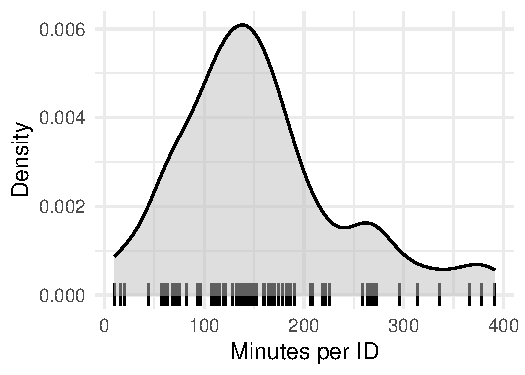
\includegraphics{Quantex_interaction_paper_files/figure-latex/quantex-minutes-per-child-1} 

}

\caption{Video recording duration (in minutes) per Child in the Quantex Dataset.}\label{fig:quantex-minutes-per-child}
\end{figure}

\subsubsection{Annotation Strategy}\label{annotation-strategy}

The dataset annotations cover four key elements: persons, faces, gaze direction, objects the child interacts with. Gaze information identifies whether a detected person's gaze is directed toward the child or not. For every detected person (or reflection of a person, such as in a mirror) and face, additional attributes like age and gender are collected. Objects are categorized into six distinct groups: book, screen, animal, food, toy, and kitchenware, with an additional category for other objects. The dataset focus is on detecting and labeling instances of (social) interaction and engagement through these key categories. The annotation strategy is displayed in Figure \ref{fig:camera-cvat-activity-classes}.

\begin{figure}

{\centering 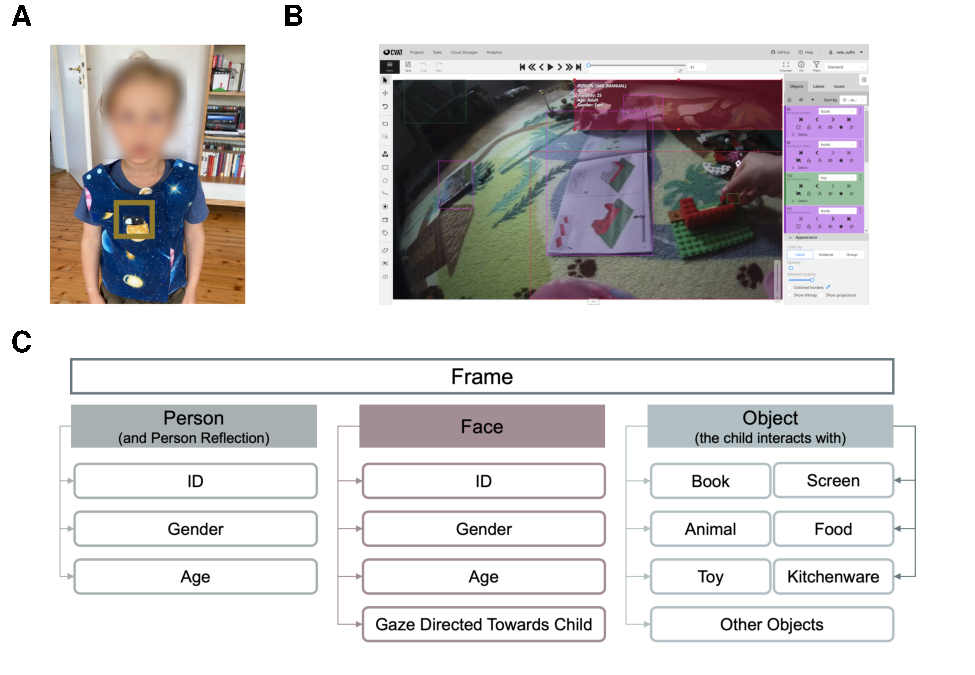
\includegraphics{Quantex_interaction_paper_files/figure-latex/camera-cvat-activity-classes-1} 

}

\caption{\textbf{A} – Vest with the embedded camera worn by the children, \textbf{B} – CVAT platform utilized for video annotation, \textbf{C} – Annotation Strategy in the Quantex dataset.}\label{fig:camera-cvat-activity-classes}
\end{figure}

\subsection{Data Collection}\label{data-collection}

This study collected egocentric video recordings from 76 children, aged 3 to 5 years, over a span of 73 months. Participating families lived in a mid-sized city in Germany. To capture the children's everyday experiences, a wearable vest equipped with a camera was used, as shown in figure \ref{fig:camera-cvat-activity-classes}. The camera, a \emph{PatrolEyes WiFi HD Infrared Police Body Camera}, provided high-definition video (1920x1080p at 30 fps) with a 140-degree wide-angle lens and also recorded audio. Children were free to move around and engage in their usual activities at home without any interference or instructions given to their parents.

\subsection{Data Preprocessing}\label{data-preprocessing}

For the video data, the annotation strategy required persons, faces, and objects to be labeled even when only partially visible, as long as key features such as facial landmarks (e.g., nose, eye, or mouth) or parts of a person or object were clearly visible. Frames that were too blurry due to movement were marked as ``noise'' and excluded from further analysis. Additionally, frames where the child was not wearing the camera, as well as any scenes containing nudity, were also labele d as noise and removed from the dataset. To prepare the video data for analysis, one frame per second was annotated, corresponding to every 30th frame in the video. Similarly, every 30th raw frame was extracted from the annotated video files. No preprocessing was applied to the audio data, which was used in its raw form for analysis.

\subsection{Automated Analysis Pipeline}\label{automated-analysis-pipeline}

\subsubsection{Person Detection}\label{person-detection}

\subsubsection{Face Detection}\label{face-detection}

\begin{table}[tbp]

\begin{center}
\begin{threeparttable}

\caption{\label{tab:face-detection-metrics}Evaluation metrics for the YOLO11 face detection model trained on the Quantex dataset.}

\begin{tabular}{llll}
\toprule
Dataset & \multicolumn{1}{c}{Precision} & \multicolumn{1}{c}{Recall} & \multicolumn{1}{c}{F1-Score}\\
\midrule
Quantex & 0.90 & 0.83 & 0.86\\
\bottomrule
\end{tabular}

\end{threeparttable}
\end{center}

\end{table}

\subsubsection{Gaze Classification}\label{gaze-classification}

\subsubsection{Voice Detection and Classification}\label{voice-detection-and-classification}

\subsection{Feature Extraction}\label{feature-extraction}

\section{Results}\label{results}

\subsection{Presence of Aspects of Social Interaction}\label{presence-of-aspects-of-social-interaction}

\subsubsection{Presence of a Person}\label{presence-of-a-person}

\subsubsection{Presence of a Face}\label{presence-of-a-face}

\subsubsection{Presence of Gaze Directed at the Child}\label{presence-of-gaze-directed-at-the-child}

\subsubsection{Presence of Language}\label{presence-of-language}

\subsection{Co-occurrence of Aspects of Social Interaction}\label{co-occurrence-of-aspects-of-social-interaction}

\section{General Discussion}\label{general-discussion}

\newpage

\section{References}\label{references}

\newpage

\section{Supplementary Material}\label{supplementary-material}

\subsection{Yolo Face Detection Model Training Details}\label{yolo-face-detection-model-training-details}

Face detection is perfored utilizing Ultralytics Yolo11 (Jocher \& Qiu, 2024)
We employed a YOLO11 model pretrained for face detection (Codd, 2024), which was fine-tuned on our dataset to adapt it to the unique characteristics of our egocentric dataset, captured using chest-mounted cameras. While we initially experimented with the MTCNN model, its performance on our dataset proved insufficient. Consequently, we chose YOLO due to its streamlined training process and fewer requirements for data preparation. The 100 annotated videos were divided into 70\% for training, 10\% for validation, and 20\% for testing. This split corresponded to 51 with 72687 frames for training, 6 videos with 7720 frames for validation, and 7 videos with 9272 frames for testing.

Model training was conducted using the Ultralytics framework (Jocher, Jing, \& Chaurasia, 2023) on a Linux server equipped with 48 cores and 187 GB of RAM. The training process utilized YOLO's built-in data augmentation, a batch size of 16, a cosine annealing learning rate scheduler, and early stopping after 10 epochs without improvement, with a maximum of 200 epochs. Training concluded after 86 epochs, achieving a precision of 0.90 and a recall of 0.83, resulting in an \(F_1\)-score of 0.86 on the testing set. This indicates strong performance in correctly identifying most faces while minimizing errors, although some challenges remain. These performance metrics, summarized in Table \ref{tab:face-detection-metrics}, underscore the model's ability to reliably detect faces, with further details and evaluation available in the supplementary materials.

The model performed well in detecting faces, particularly when fully visible from the front, but few challenges remain in more dynamic scenarios. For example, faces that are partially visible, rotated, or seen from the side often resulted in detection errors. Furthermore, false negatives were more common when faces were occluded by the child's body, blurred due to movement, or situated in the background. While background faces are less relevant, as they are unlikely to be part of an interaction with the child, missed detections due to occlusions or motion blur present a greater challenge. In these cases, we rely on adjacent frames to provide clearer views for more accurate classification. These difficulties underscore the challenges of working with egocentric video data, where dynamic movement and varying perspectives, typical of chest-mounted camera recordings, introduce additional complexity.

Accurate face detection remains a crucial step in our automated analysis pipeline, as it serves as the foundation for subsequent gaze classification. Identifying the presence and position of faces ensures that gaze direction can be reliably analyzed, allowing us to determine when and how individuals engage with the child.

\subsubsection{Model Training Details}\label{model-training-details}

\begin{figure}

{\centering 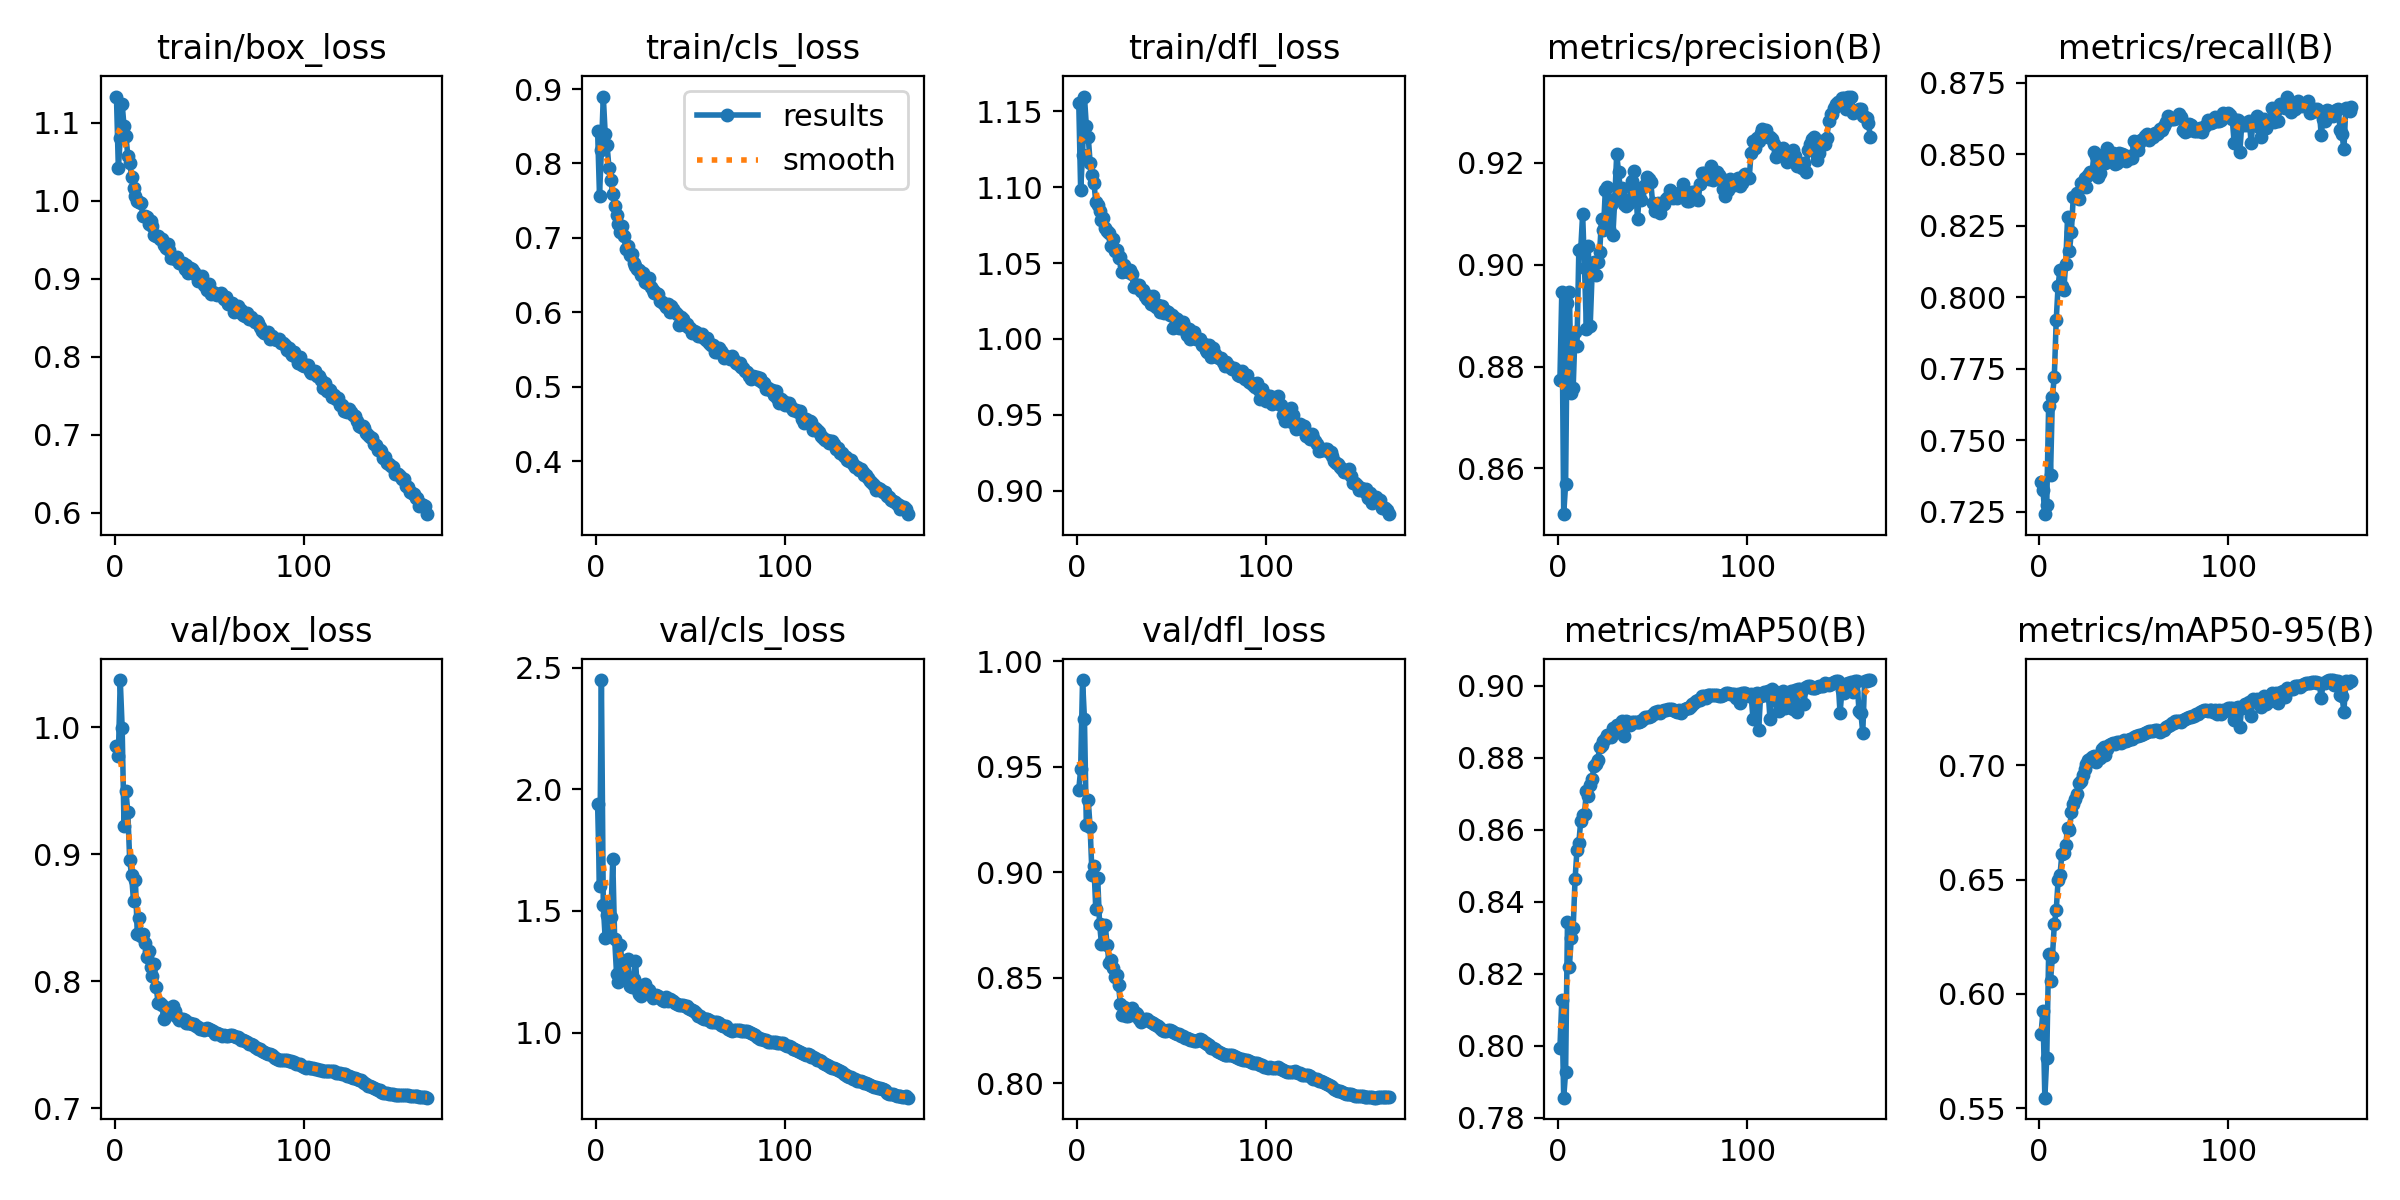
\includegraphics[width=300px]{images/yolo_face_loss_curves} 

}

\caption{Training and Validation Loss Curves for the YOLO11 face detection model.}\label{fig:face-loss-curves}
\end{figure}

\begin{itemize}
\item
  Yolo11 uses a loss function consisting of three components: box loss, class loss, and distribution focal loss (DFL) as displayed in \ref{fig:face-loss-curves} (Codd, 2024).
\item
  Box Loss: difference between expected bounding boxes and ground truth boxes.
\item
  Class Loss (Cls Loss): Measures the model's ability to accurately identify detected items which is less relevant in our case as we are only interested in one class: faces
\item
  Distribution Focal Loss (DFL) improves the model's ability to identify difficult-to-detect objects or classes
\item
  we can see that during training all three loss components decrease over time, indicating that the model is learning and improving its performance.
\item
  more precisely, decrease in box loss indicates that the model is becoming more precise at localizing items within images, classification loss converges quickly showing that the model is able to identify faces accurately, and the distribution focal loss decreases over time, indicating that the model is learning to focus on difficult-to-detect objects or classes, improving its overall performance.
\end{itemize}

\subsubsection{Model Evaluation Metrics}\label{model-evaluation-metrics}

Jocher (2024)

\begin{figure}

{\centering 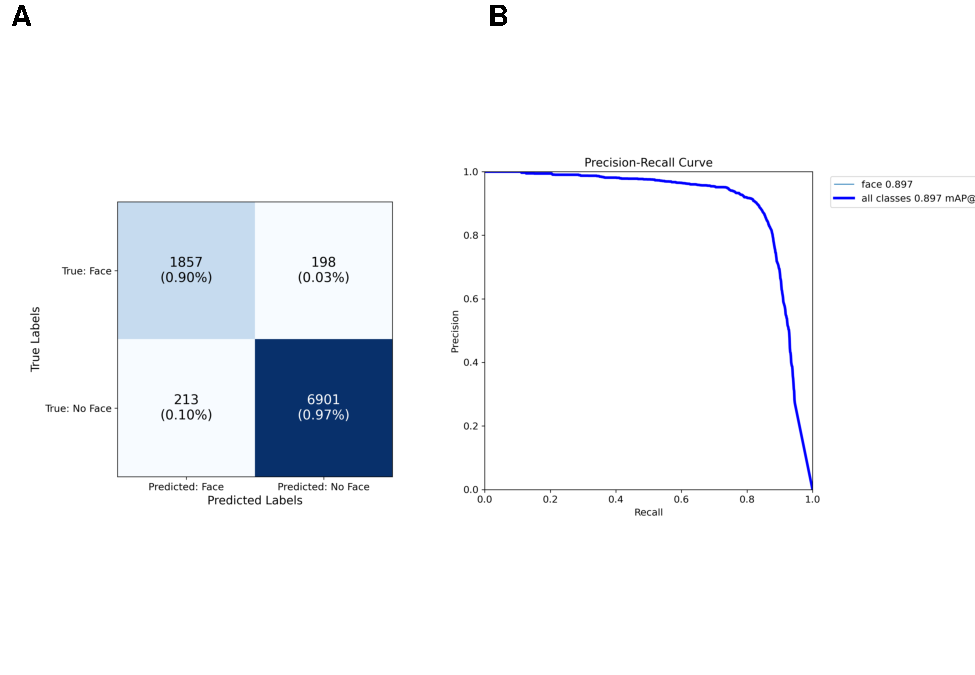
\includegraphics{Quantex_interaction_paper_files/figure-latex/face-metrics-1} 

}

\caption{Evaluation metrics for the YOLO11 face detection model trained on the Quantex dataset.}\label{fig:face-metrics}
\end{figure}

\begin{itemize}
\tightlist
\item
  when looking at confusion matrix: you can see that the majority of images are correctly identified as face. 0.86\% of all faces are correctly identified by the model, resulting in a total of 1000 faces detected, while r num\_faces\_missed` weren't detected.
\item
  looking into those false negative cases (meaning model predicts no face but label says face): we can see that the majority of those cases are due to three reasons: faces in the background, blurry faces or faces that are occluded by the child's body.
\item
  (\textbf{ref?})(fig:face-metrics) provides examples of correctly classified face images (true positives) and incorrectly classified face images (false negatives).
  Regarding images in the background were less concerned as they are unlikely to be part of an interaction with the child. However, the other two cases are more critical as they are likely to be part of an interaction with the child.
\item
  here we have to rely on the surrounding frames that hopefully contain a clearer view of the face to make a more accurate classification.
\item
  a small amount of images are classified as faces while no face is present in the image (false positive). from the confusion matrix you can derive that the model only classifies 0.86 images, corresponding to
\end{itemize}

This is due to the model's tendency to detect faces in objects that resemble faces, such as toys or drawings.

\begin{itemize}
\tightlist
\item
  when looking at the precision-recall curve: we can see that the model performs well in terms of precision and recall, with a high precision and recall value, indicating that the model is able to detect faces accurately and with high confidence.
\item
  the curve stays close to the top left corner, indicating that the model is able to detect faces with high precision and recall, which is crucial for our analysis pipeline.
\end{itemize}

\begin{enumerate}
\def\labelenumi{\arabic{enumi}.}
\setcounter{enumi}{3}
\item
  Model Hyperparameter Settings and Tuning
  • Hyperparameter Search Results: If you did any hyperparameter tuning (e.g., batch size, learning rate), you could include a plot showing how different values impacted performance.
  • Plot type: A heatmap or line plot showing the effect of different hyperparameter combinations on a given metric (e.g., F1-score).
\item
  Training Time and Hardware Utilization
  • Training Time Breakdown: Include the total time taken for training and the hardware specifications (e.g., time per epoch, total training time).
  • Plot type: A bar graph showing training time per epoch or the total time required for training.
  • Resource Utilization (optional): If you tracked resource usage during training (e.g., GPU/CPU utilization, memory usage), you can provide plots to show how efficiently the hardware was used.
  \newpage
\end{enumerate}

\begingroup
\setlength{\parindent}{-0.5in}
\setlength{\leftskip}{0.5in}

\phantomsection\label{refs}
\begin{CSLReferences}{1}{0}
\bibitem[\citeproctext]{ref-coddYOLOv11nfacedetection2024}
Codd, A. (2024). \emph{{YOLOv11n-face-detection}}. Retrieved from \url{https://huggingface.co/AdamCodd/YOLOv11n-face-detection}

\bibitem[\citeproctext]{ref-jocherUltralyticsYolo11Performance2024}
Jocher, G. (2024). \emph{Ultralytics {Yolo11 Performance Metrics}}. Retrieved from \url{https://docs.ultralytics.com/guides/yolo-performance-metrics/?utm_source=chatgpt.com}

\bibitem[\citeproctext]{ref-jocherUltralyticsYOLO2023}
Jocher, G., Jing, Q., \& Chaurasia, A. (2023). \emph{Ultralytics {YOLO}}. Retrieved from \url{https://github.com/ultralytics/ultralytics}

\bibitem[\citeproctext]{ref-jocherUltralyticsYOLO112024}
Jocher, G., \& Qiu, J. (2024). \emph{Ultralytics {YOLO11}}. Retrieved from \url{https://github.com/ultralytics/ultralytics}

\end{CSLReferences}

\endgroup

\newpage

\section{Appendix}\label{appendix}


\end{document}
